\chapter{How I Turned \texorpdfstring{\$1,000}{1000 Dollars} Into \texorpdfstring{\$1 Billion}{1 Billion Dollars}}

The episode begins with the conclusion before the proof. Glen Boyd reports a product pivot that did \(\$50{,}000\) in its first month without advertising, nearly caught the older security business within eleven months, and reached \(\$120{,}000{,}000\) in sales within four years. The notes below treat the interview as evidence for a business mechanism: not a formula for wealth, but a sequence of ownership, risk, customer proof, financing discipline, and scale.

\section{The Result Before The Mechanism}

The opening numbers are the hook. Before we know the first product, the team, or the market, we are given the growth trace:
\begin{equation}
\$50{,}000\ \text{in month 1}
\;\longrightarrow\;
\text{near the old security business by month 11}
\;\longrightarrow\;
\$120{,}000{,}000\ \text{in sales by year 4}.
\end{equation}

This is not yet an explanation. It is a target. The question is what mechanism could turn a small technical company into something that scaled so quickly.

Boyd then backs up. He had taught himself programming, started young, and built EG Software, an early technology company that he later took public in 1999 and sold in a merger. The first important detail is that the billion-dollar outcome did not begin as a billion-dollar idea. It began as a narrowly useful product in a narrowly defined market.

\section{From Security Logs To Marketing Signals}

The original product was not web analytics. Boyd describes it as a security product for local-area networks, a kind of surveillance and audit-control system for internal networks. Banks and financial institutions needed ways to see what was happening as more work became computerized. The product logged and analyzed traffic and access inside a network.

In mechanism form, the first business looked like this:
\begin{equation}
\text{local-area-network traffic}
\;\longrightarrow\;
\text{logging and analysis}
\;\longrightarrow\;
\text{security or audit report}.
\end{equation}

That was already a real business. Boyd says the small team had the Federal Reserve, almost every major bank in the United States, and a four-person operation doing roughly \(\$1{,}000{,}000\) a year from a small office. The important thing is that the company owned a working capability: rapid analysis of large amounts of traffic data.

Then the internet arrived. Yahoo and Netscape had gone public, and Boyd says he realized the world was becoming networked. The market changed faster than the product category. So the business question became: what happens if the same analysis engine is pointed at a new kind of traffic?

\begin{figure}
\centering
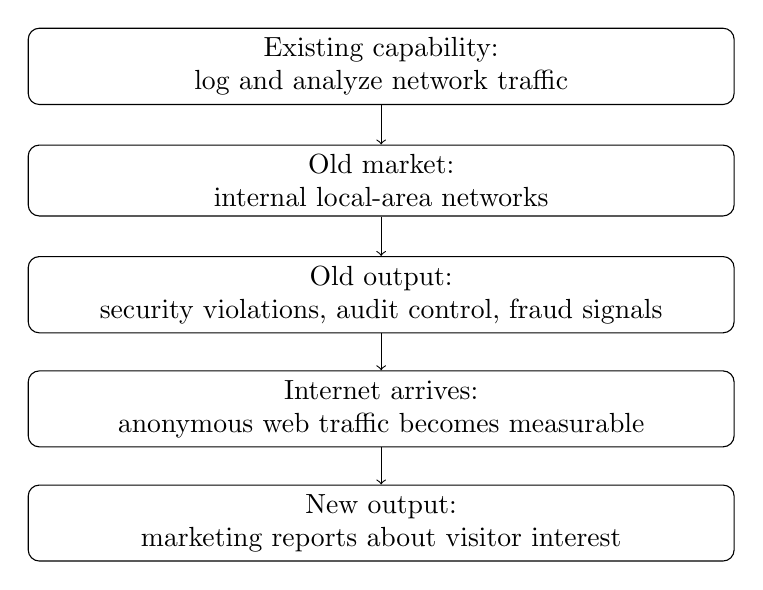
\begin{tikzpicture}[x=1cm,y=1cm]
\node[draw, rounded corners, align=center, text width=.72\linewidth] (a) at (0,0) {Existing capability:\\log and analyze network traffic};
\node[draw, rounded corners, align=center, text width=.72\linewidth] (b) at (0,-1.45) {Old market:\\internal local-area networks};
\node[draw, rounded corners, align=center, text width=.72\linewidth] (c) at (0,-2.90) {Old output:\\security violations, audit control, fraud signals};
\node[draw, rounded corners, align=center, text width=.72\linewidth] (d) at (0,-4.35) {Internet arrives:\\anonymous web traffic becomes measurable};
\node[draw, rounded corners, align=center, text width=.72\linewidth] (e) at (0,-5.80) {New output:\\marketing reports about visitor interest};
\draw[->] (a) -- (b);
\draw[->] (b) -- (c);
\draw[->] (c) -- (d);
\draw[->] (d) -- (e);
\end{tikzpicture}
\caption{The pivot was not from nothing to something; it was from one use of a data-analysis engine to another.}
\end{figure}

The pivot can be written compactly:
\begin{align}
\text{security product}
&:\quad
\text{local traffic} \longrightarrow \text{security report},\\
\text{web analytics product}
&:\quad
\text{anonymous web traffic} \longrightarrow \text{marketing report}.
\end{align}

This is the first commercial lesson of the interview. A product may look like a single thing, but underneath it there may be a more general machine.

\subsection{Question \& Answer}

\paragraph{Question.}
How did Boyd know that this was the company, and the idea, to go all in on?

\paragraph{Answer.}
He did not know in the sense of proof. He saw a historical discontinuity. The old local-area-network world was being replaced by a networked world. His train metaphor matters: the internet was passing by, and if they ran fast enough, they might catch the last car.

The resolution comes only after the pivot. They changed the target from fraud and audit control to anonymous web behavior. Early customers such as Sports Illustrated needed to know whether a website had \(100{,}000\) visitors or \(10{,}000\) visitors returning ten times. Boyd already had technology that could analyze large data streams quickly. The market supplied the proof:
\begin{equation}
\text{old analysis engine} + \text{new internet traffic}
\;\Longrightarrow\;
\text{new market}.
\end{equation}

\section{The Adoption Test}

When the interviewer asks about funding, Boyd does not begin with pitch decks or investor language. He begins with demonstration. Ideas are hard to fund; something that can be shown is easier. Better still is a product, even a partial product, that people are already using.

He calls this the dog-food test: will people actually use the product? In our notation, the funding rule is not a theorem, but it is a useful operating inequality:
\begin{equation}
\text{idea}
\;<\;
\text{demonstrable product}
\;<\;
\text{product with early adoption}.
\end{equation}

A more explicit version is:
\begin{equation}
\text{idea}
+
\text{demonstrable product}
+
\text{early adoption}
\;\Longrightarrow\;
\text{credible funding path}.
\end{equation}

\paragraph{Worked example.}
Suppose two founders ask for capital.

\begin{enumerate}
\item Founder A has only a verbal claim: ``people will want this.''
\item Founder B has a small working product and a small group of users.
\item Founder C has the same working product, repeated usage, and evidence that users are gravitating toward it without heavy advertising.
\end{enumerate}

The investor uncertainty decreases in that order:
\begin{equation}
U_A > U_B > U_C,
\end{equation}
where \(U\) denotes uncertainty about whether the product has demand. Boyd's point is that early use is not just a vanity signal. It changes the financing conversation because it answers the first practical question: whether the market wants the thing.

\section{Risk, Partnership, And Survival Runway}

The risk story is concrete. Boyd had a newborn on the way, quit his job, started writing the first product, and got down to about \(\$1{,}000\) in the bank. He sold his motorcycle, extending the runway by another month or two. Then his partner came in and put personal money into the company.

The early survival equation is rough but faithful:
\begin{equation}
\$1{,}000\ \text{left}
+
\text{motorcycle sale}
+
\text{partner cash}
\;\longrightarrow\;
\text{enough runway to continue}.
\end{equation}

The risk was not romanticized. Boyd's fallback model was simple: if it failed, he would get a job. That fallback made the risk mentally survivable. The regret model was also simple: if he did not try, he would sit at a job wondering why he had not tried.

The partner theme returns later when he talks about work-life balance. A strong co-partner was not merely emotional support. It was an operating structure: division of labor, emergency backup, complementary or even non-complementary skills, and enough trust to argue without breaking the business.

\section{Bad Fit, Venture Capital, And Ownership}

Boyd contrasts two financial decisions. The bad one was entering a business he did not want to be in. He describes a construction loan, collateral, failing management, several years spent turning things around, a tragic accident, and a loss close to \(\$3{,}000{,}000\). The rule he extracts is not abstract: do not get involved in something you do not want to be involved in, especially when your instinct says no.

Then comes the counterintuitive ``best'' financial decision. The company was profitable and growing fast, but Boyd and his partner wanted additional capital to expand faster. They courted a venture-capital firm. The process took attention and energy. In the end the firm passed.

\begin{figure}
\centering

\includegraphics[width=\linewidth]{lecture_16_figure_05.png}
\caption{Startup-pitch imagery near Boyd's account of courting venture capital. The frame is contextual b-roll; the ownership mechanism comes from the spoken interview, not from the small unreadable charts on the board.}
\end{figure}

\subsection{Question \& Answer}

\paragraph{Question.}
Why would a failed financing process become the best financial decision?

\paragraph{Answer.}
Because the failure changed the ownership equation. Without venture capital, they lacked the financial cushion they wanted. But that forced frugality, and it preserved founder ownership. Boyd says that when they took the company public, he and his partner owned \(95\%\) of it.

\begin{figure}
\centering
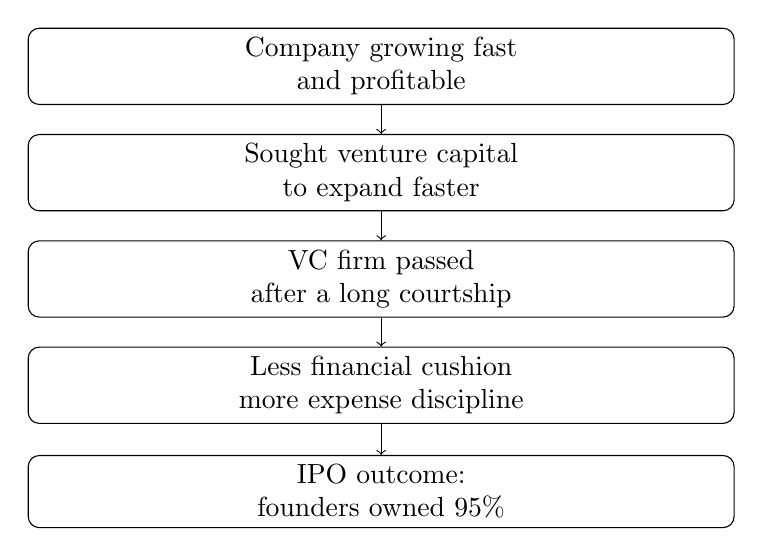
\begin{tikzpicture}[x=1cm,y=1cm]
\node[draw, rounded corners, align=center, text width=.72\linewidth] (a) at (0,0) {Company growing fast\\and profitable};
\node[draw, rounded corners, align=center, text width=.72\linewidth] (b) at (0,-1.35) {Sought venture capital\\to expand faster};
\node[draw, rounded corners, align=center, text width=.72\linewidth] (c) at (0,-2.70) {VC firm passed\\after a long courtship};
\node[draw, rounded corners, align=center, text width=.72\linewidth] (d) at (0,-4.05) {Less financial cushion\\more expense discipline};
\node[draw, rounded corners, align=center, text width=.72\linewidth] (e) at (0,-5.40) {IPO outcome:\\founders owned \(95\%\)};
\draw[->] (a) -- (b);
\draw[->] (b) -- (c);
\draw[->] (c) -- (d);
\draw[->] (d) -- (e);
\end{tikzpicture}
\caption{The rejected financing round becomes valuable because it preserves ownership and forces frugality.}
\end{figure}

The compact mechanism is:
\begin{equation}
\text{sought VC}
\;\longrightarrow\;
\text{VC passed}
\;\longrightarrow\;
\text{frugality}
\;\longrightarrow\;
95\%\ \text{founder ownership at IPO}.
\end{equation}

\section{Scaling Until People Run Out Of Oxygen}

The advice on scaling begins with expenses: as the business scales, expenses scale too. One bad dip can wipe out the company if costs have outrun resilience. But the more distinctive part of Boyd's scaling advice comes from his reading of \emph{Into Thin Air}.

The metaphor is altitude. At a certain height, even tying one's shoes becomes difficult. People have different capacities. Some can go higher; some need supplemental oxygen; some must go down the mountain. Boyd maps this directly onto a fast-growing company. An employee who was excellent six months earlier may be failing because the job has changed faster than the person can adapt.

A manager hired to handle \(4\text{--}10\) people may suddenly be managing \(20\text{--}30\):
\begin{equation}
4\text{--}10\ \text{direct reports}
\;\longrightarrow\;
20\text{--}30\ \text{direct reports}
\;\longrightarrow\;
\text{capacity failure risk}.
\end{equation}

The operating rule is an update rule for hiring and responsibility:
\begin{align}
\text{current role} &= R,\\
\text{near-future role} &= R + \Delta R,\\
\text{hire for capacity} &\geq R + \Delta R.
\end{align}

That is the reason Boyd changed hiring practices. If the company would need someone to manage \(50\) people within a year, it was not enough that the candidate could manage \(20\) now. He wanted someone who had already been up the mountain.

\begin{table}
\centering
\begin{tabular}{|p{.24\linewidth}|p{.28\linewidth}|p{.36\linewidth}|}
\hline
\textbf{Growth state} & \textbf{Failure signal} & \textbf{Management response} \\
\hline
Employee succeeds at current scale & Work remains manageable & Keep responsibility matched to role \\
\hline
Company grows rapidly & Same person now carries a much larger span & Stop adding balls; reduce or divide responsibility \\
\hline
Future role is predictable & Candidate has not operated at that altitude & Hire above the current level \\
\hline
\end{tabular}
\caption{Boyd's altitude metaphor converted into an operating table for scaling responsibility.}
\end{table}

\section{Money, Time, And The Last Constraint}

After the sale, the interviewer asks whether money buys happiness. Boyd's answer is deliberately bounded. Money does buy some happiness when it moves a person from poverty toward security: paying bills, sending children to college, and gaining freedom to try new things. But beyond a point, the champagne does not get better, the beaches do not get nicer, and more money does not keep buying more happiness.

That claim can be expressed as a saturating curve rather than a straight line:
\begin{equation}
\text{security value of money}
\quad
\text{rises quickly at low wealth, then flattens after basic freedom is reached.}
\end{equation}

The younger-self advice follows the same logic. Enjoy life more. Protect health earlier. Build deeper relationships. Do not spend too much once money arrives. Get serious financial advice.

The final rule is about time. Boyd says procrastination is the enemy because time is not renewable. If one is going to fail, fail fast, learn, and move on. For an entrepreneur, delay is not neutral:
\begin{equation}
\text{delay}
\;\longrightarrow\;
\text{later failure or later learning}
\;\longrightarrow\;
\text{greater distance from success}.
\end{equation}

\section{Summary}

The chapter's spine is a sequence of commercial transformations. A small security company owned a useful analysis engine. The internet changed the field of application. A security report became a marketing report, and early customers validated the new use. Funding became less about the idea and more about demonstrated use. Risk became survivable because Boyd had a fallback, a partner, and enough runway to keep going. The rejected venture-capital round became valuable because it preserved ownership and forced discipline. Scaling then revealed a different bottleneck: people can run out of managerial oxygen as the company climbs.

The practical lesson is not that every founder should copy Boyd's path. It is that wealth in this interview is built through a chain:
\begin{equation}
\text{technical capability}
\;\longrightarrow\;
\text{market pivot}
\;\longrightarrow\;
\text{customer validation}
\;\longrightarrow\;
\text{disciplined financing}
\;\longrightarrow\;
\text{retained ownership}
\;\longrightarrow\;
\text{durable wealth}.
\end{equation}